\section{Auswertung} \label{sec:Auswertung}
\subsection{Aufgabenteil a)}
\label{sec:AufgabeA}
% Zunächst sollten zwei unbekannte Ohm'sche Widerstände mithilfe der Wheatstoneschen Brückenschaltung ausgemessen werden.
% Aber wir nur einen vermessen – was wir besser nicht erwähnen ;)
Zunächst sollte ein unbekannter Ohm'sche Widerstand (\enquote{Wert 13}) mithilfe der \hyperref[sec:Wheatstone]{Wheatstoneschen Brückenschaltung} ausgemessen werden.
Für die Linearität $\frac{R_3}{R_4}$ gilt eine unsystematische Abweichung von $\pm 0.5 \%$.
Für den festen Widerstand $R_2$ war dagegen keine Abweichung angegeben, sodass die berechnete Abweichung für $R_x$ kaum aussagekräftig ist.

Die folgende Tabelle ist in je zwei Zeilen untergliedert, weil der Versuch mit einem anderen Potentiometer wiederholt wurde.

\begin{table}
\centering
% \caption{IMPROVE}
\begin{tabular}{c c c c}
\toprule
$R_2 \mathbin{/} \si{\ohm}$ &
$R_3 \mathbin{/} \si{\ohm}$ &
$R_4 \mathbin{/} \si{\ohm}$ &
$R_x \mathbin{/} \si{\ohm}$ \\
\midrule
664	& 317 &	683	&	308.182 \pm 1.541 \\
332	& 483 &	517	&	310.166 \pm 1.551 \\
\midrule
332	& 488 &	512	&	316.438 \pm 1.582 \\
664	& 323 &	677	&	316.798 \pm 1.584 \\
\bottomrule
\end{tabular}
\end{table}

Damit ist $R_x$ zu $312.896 \pm 0.782$ bestimmt.

\subsection{Aufgabenteil b)}
\label{sec:AufgabeB}
Mithilfe der \hyperref[sec:Kapazität]{Kapazitätsmessbrücke} sollte eine unbekannte Kapazität (\enquote{Wert 9}) bestimmt werden.
Die Toleranz (Eichgenauigkeit) des Verlustwiderstands beträgt hier $\pm \SI{3}{\percent}$.
Wie zuvor wird die Abweichung für $\frac{R_3}{R_4}$ berücksichtigt.

\begin{table}
  \centering
  % \caption{IMPROVE}
  \begin{tabular}{c c c c c c}
    \toprule
    $C_2 \mathbin{/} \si{\nano\farad}$ &
    $R_2 \mathbin{/} \si{\ohm}$ &
    $R_3 \mathbin{/} \si{\ohm}$ &
    $R_4 \mathbin{/} \si{\ohm}$ &
    $C_x \mathbin{/} \si{\nano\farad}$ &
    $R_x \mathbin{/} \si{\ohm}$ \\
    \midrule
    750 &	267   & 630 & 370 & 440.476 \pm 2.202 & 454.622 \pm 13.827 \\
    450 & 438.5 & 508 & 492 & 435.827 \pm 2.179 & 452.760 \pm 13.770 \\
    \bottomrule
  \end{tabular}
\end{table}

\ \\
Die gemittelten Werte sind
$C_x = \SI{438.151 \pm 1.549}{\nano\farad}$
und
$R_x = \SI{453.691 \pm 9.757}{\ohm}$.

\subsection{Aufgabenteil c)}
Mit der \hyperref[sec:Induktivität]{Induktivitätsbrücke} soll eine unbekannte Induktivität (\enquote{Wert 17}) berechnet werden.
Die Toleranz des Verlustwiderstands entspricht der aus \hyperref[sec:AufgabeB]{b)}.

% TODO: uncertainties checken, siehe TODONEW

\begin{table}
  \centering
  % \caption{IMPROVE}
  \begin{tabular}{c c c c c c}
    \toprule
    $L_2 \mathbin{/} \si{\milli\henry}$ &
    $R_2 \mathbin{/} \si{\ohm}$ &
    $R_3 \mathbin{/} \si{\ohm}$ &
    $R_4 \mathbin{/} \si{\ohm}$ &
    $L_x \mathbin{/} \si{\milli\henry}$ &
    $R_x \mathbin{/} \si{\ohm}$ \\
    \midrule
    27.5 & 57 & 605.5 & 394.5 & 42.208 \pm 0.211 & 87.487 \pm 0.437 \\
    14.6 & 33 & 740.5 & 259.5 & 41.662 \pm 0.208 & 94.168 \pm 0.471 \\
    \bottomrule
  \end{tabular}
\end{table}

\ \\
Die gemittelten Werte sind
$L_x = \SI{41.935 \pm 0.148}{\milli\henry}$ und
$R_x = \SI{90.827 \pm 0.321}{\ohm}$.

\subsection{Aufgabenteil d)}
Hier soll der \enquote{Wert 17} erneut berechnet werden, allerdings mit einer \hyperref[sec:Maxwell]{Maxwell-Brücke}.
Die Toleranz für $R_3$ und $R_4$ beträgt wieder $\pm 3\%$.

\begin{table}
  \centering
  % \caption{IMPROVE}
  \begin{tabular}{c c c c c c}
    \toprule
    $R_2 \mathbin{/} \si{\ohm}$ &
    $R_3 \mathbin{/} \si{\ohm}$ &
    $R_4 \mathbin{/} \si{\ohm}$ &
    $C_4 \mathbin{/} \si{\nano\farad}$ &
    $L_x \mathbin{/} \si{\milli\henry}$ &
    $R_x \mathbin{/} \si{\ohm}$ \\
    \midrule
    664	&  81.5	& 608  & 750 & 40.587 \pm 1.218 & 89.007 \pm 3.776 \\
    664	& 137.5	& 1003 & 450 & 41.085 \pm 1.233 & 91.027 \pm 3.862 \\
    332	& 277.5	& 1003 & 450 & 41.459 \pm 1.244 & 91.854 \pm 3.897 \\
    \bottomrule
  \end{tabular}
\end{table}

\ \\
Die gemittelten Werte sind
$L_x = \SI{41.0435 \pm 0.711}{\milli\henry}$
und
$R_x = \SI{90.629 \pm 2.220}{\ohm}$.

\subsection{Aufgabenteil e)}
\label{sec:AufgabeE}

In dieser Messreihe wurde die Abhängigkeit der Brückenspannung von der Frequenz für eine \hyperref[sec:WR]{Wien-Robinson-Brücke} untersucht.
Das folgende Diagramm zeigt den Verlauf der Spannung.
Auf der x-Achse ist $\Omega = \frac{v}{v_0}$ aufgetragen, wobei $v_0$ die Frequnz dargestellt, bei
der die Brückenspannung $U_\text{Br}$ miminal wird.
Auf der y-Achse ist der Quotient $\frac{U_\text{Br}}{U_\text{S}}$ dargestellt.
Die Theoriekurve wurde mithilfe von \autoref{eqn:WienRobinsonBrNachS} berechnet.

\begin{table}
  \centering
  % \caption{IMPROVE}
  \begin{tabular}{c c}
    \toprule
    $\nu$ \,/\, \si{\hertz} &
    $U_\text{Br}$ \,/\, \si{\volt} \\
    \midrule
    20  & 3.12  \\
    40  & 2.88  \\
    80  & 2.1   \\
    160 & 0.77  \\
    215 & 0.17  \\
    220 & 0.141 \\
    221 & 0.136 \\
    222 & 0.133 \\
    223 & 0.13  \\
    224 & 0.128 \\
    225 & 0.127 \\
    226 & 0.125 \\
    227 & 0.126 \\
    228 & 0.127 \\
    229 & 0.127 \\
    230 & 0.13  \\
    300 & 0.625 \\
    320 & 0.75  \\
    480 & 1.55  \\
    640 & 2.04  \\
    \bottomrule
  \end{tabular}
\end{table}


% IMPROVE: verhindere das Floaten durch Verzicht auf figure…
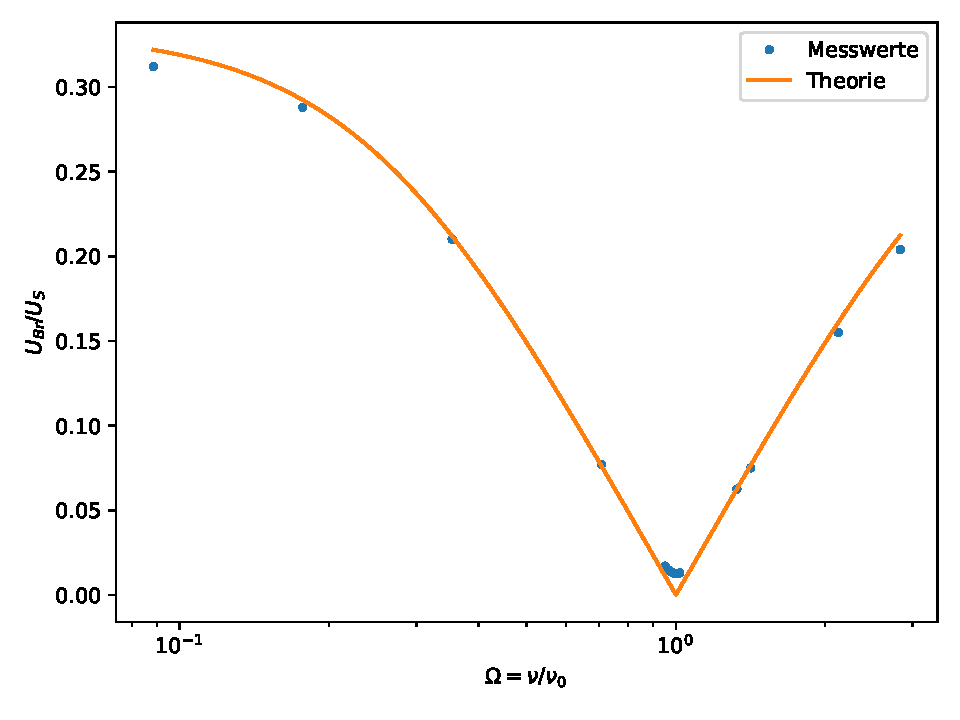
\includegraphics[scale=0.8]{build/plot1.pdf}
\ \\
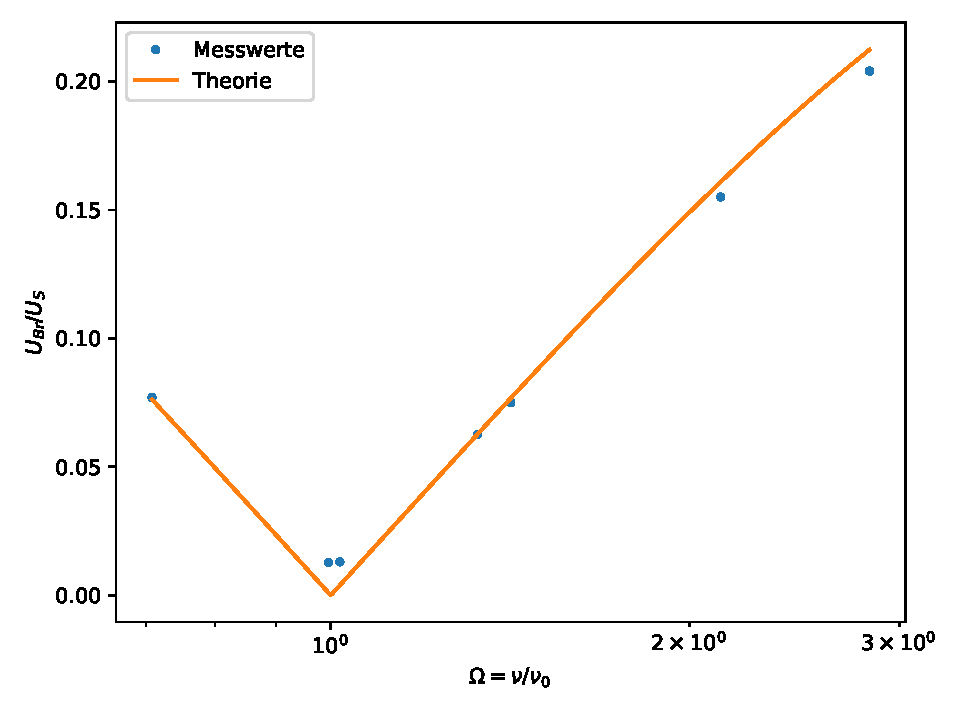
\includegraphics[scale=0.5]{build/plot2.pdf}
\ \\
Wie im Diagramm zu erkennen ist, stimmen Messswerte und Theorie gut überein.
Lediglich das Minimum ist nicht so ausgeprägt wie in der Theorie – was direkt zur \hyperref[sec:KlirrfaktorAuswertung]{Klirrfaktor-Messung} führt.

\subsection{Aufgabenteil f)}
\label{sec:KlirrfaktorAuswertung}

In diesem Aufgabenteil soll der sogenannte Klirrfaktor $k$ nach der Formel
\begin{equation}
     k := \frac{\sqrt{U_2^2 + U_3^2 + ...}}{U_1}
\end{equation}
berechnet werden.
Vereinfachend wird angenommen, dass die Summe der Oberwellen nur aus der zweiten Oberwelle (mit Frequenz $2\omega_0$) besteht, also
\begin{equation}
     k = \frac{\sqrt{U_2^2}}{U_1} = \frac{U_2}{U_1}
\end{equation}
gilt.
\ \\
$U_1$ bezeichnet hierbei die Amplitude der Grundwelle der Speisespannung $U_\text{S}$ und $U_2$ die der zweiten Oberwelle.
Um $U_2$ zu berechnen, wird der Zusammenhang aus \eqref{eqn:WienRobinsonBrNachS} verwendet
und $\Omega = \frac{\omega}{\omega_0} = 2$ eingesetzt:
\begin{equation}
  f(2)
  := \left\lvert \frac{U_\text{Br}}{U_\text{S}} \right\rvert
  =  \sqrt{ \frac{1}{9} \frac{(2^2 - 1)^2}{(1 - 2^2)^2 + 9 \cdot 2^2} }
  % =  0.14907119849998599
  =  0.1491
\end{equation}

Dann ist
\begin{equation*}
  U_2
  % := \lvert U_\text{S} \rvert
  = \frac{U_\text{Br}}{f(2)}
  = \frac{\SI{0.125}{\volt}}{\num{0.1491}}
  = \SI{0.8385}{\volt}
  \; ,
\end{equation*}

$U_1 = \SI{10}{\volt}$ die für $\omega=\omega_0=\SI{226}{\hertz}$ gemessene Amplitude der Grundwelle,
\ \\
und letztlich
\begin{equation*}
  k
  = \frac{U_2}{U_1}
  = \frac{\SI{0.8385}{\volt}}{\SI{10}{\volt}}
  % = 0.0838525492
  = \num{0.083852}
\end{equation*}
\ \\
der Klirrfaktor.
